%------------------------------------------------------------------------
% Chapter:  File formats
%------------------------------------------------------------------------

\chapter{File formats \label{file}}
\section{PDF data files \label{file_pdf}}

The file format for observed as well as calculated PDFs used by
{\it PDFFIT} are simple text files of the following general format
per data point:

\begin{quote}
  {\it r $\cdot$ G(r) $\cdot$  $\sigma(r)$ $\cdot$ $\sigma(G(r))$}
\end{quote}

Each data point is on a separate line in the file. The first column
contains the value of $r$ given in units of \AA. The second column
is $G(r) = 4 \pi r [\rho(r) - \rho_{0}]$ in units of \AA$^{-2}$. The
third column is ignored by {\it PDFFIT} but is required to be
compatible with the plot program {\it KUPLOT} where it takes the
value of the standard deviation of $r$. The last column contains the
standard deviation of $G(r)$ which is used to calculate the weight
$w(r)$ according to $w(r) = 1/\sigma^{2}(G(r))$. A short listing of
a PDF file is shown below:

\begin{MacVerbatim}
     0.020000    11.687810      0.0       0.081738
     0.040000    22.659353      0.0       0.155914
     0.060000    31.915903      0.0       0.212270
        :
    19.960000   -14.941482      0.0       0.162837
    19.980000   -14.858703      0.0       0.163509
    20.000000   -14.135623      0.0       0.164080
\end{MacVerbatim}

As one can see, column 3 is just occupied by some dummy number.
However, the current version of {\it PDFFIT} will also read
two-column files ($r G(r)$) and three-column files ($r G(r) w(r)$).
In order to save disk space, archived files might be compressed
using e.g. {\tt gzip}. The results can be plotted using {\it KUPLOT}
or any other visualization software that can import ASCII files.

%------------------------------------------------------------------------

\section{Structure files \label{file_stru}}

The program {\it PDFFIT} uses a keyword driven structure file format
similar to the one used by {\it DISCUS}. However, the philosophy of
{\it DISCUS} is based on simulating large disordered structures. Thus
{\it DISCUS} does not support site occupancies and includes only an
isotropic temperature factor. Furthermore, {\it PDFFIT} calculates
standard deviations for its structural parameters which need to be
saved as well. We will have a look at the $Ni$ structure files used
in the last section. The {\it DISCUS} version of this file looks like
this:

\begin{MacVerbatim}
    title Ni
    spcgr P1
    cell  3.520323,    3.520323,    3.520323,   90.0,   90.0,   90.0
    ncell 1,1,1, 4
    atoms
    NI      .000000   .000000   .000000     0.4070
    NI      .000000   .500000   .500000     0.4070
    NI      .500000   .000000   .500000     0.4070
    NI      .500000   .500000   .000000     0.4070
\end{MacVerbatim}

The file contains a title, the space group and lattice parameters in
the first three lines. The lattice parameters are again given in
units of \AA. Some explanation needs to be given concerning the
space group. The program {\it PDFFIT} ignores the space group and
just stores it to write it back in the output file. Thus no
symmetrically equivalent atom positions are created using the space
group symbol and there are no symmetry restrictions during the
refinement unless coded in the refinement parameter definitions. A
convenient way to handle systems with many symmetrically equivalent
positions is to create a similar file with the correct space group
symbol and read it with {\it DISCUS} as a {\tt cell} file. This will
generate all required positions and when saving it as a {\tt stru}
file, all positions are saved and can be read by {\it PDFFIT}. The
{\tt ncell} keyword in the input file above specifies the number of
unit cells in $x,y$ and $z$-direction and the number of atoms within
one unit cell. This way it is possible to construct a model using a
supercell based on several basic unit cells without having to change
the metric. The last keyword needs to be {\tt atoms} followed by a
list of atoms. Each line contains the atom name, the position in
fractional coordinates and the isotropic temperature factor B (see
below). When using more than one unit cell, the fractional
coordinates range from $-N/2$ to $N/2$ for $N$ unit cells. The atom
list must follow a specific order outlined in the {\it DISCUS}
manual. \par

\begin{MacVerbatim}
    title  Ni
    format pdffit
    scale  1.4875
    spcgr  P1
    cell   3.520144,  3.520144,  3.520144, 90.000000, 90.000000, 90.000000
    dcell  0.000031,  0.000031,  0.000031,  0.000000,  0.000000,  0.000000
    ncell  1,1,1, 4
    atoms
    NI      0.00000000        0.00000000        0.00000000       1.0000
            0.00000000        0.00000000        0.00000000       0.0000
            0.00501998        0.00501998        0.00501998
            0.00000515        0.00000515        0.00000515
            0.00000000        0.00000000        0.00000000
            0.00000000        0.00000000        0.00000000
\end{MacVerbatim}

This is the corresponding file in {\it PDFFIT} format. Only one $Ni$
atom is shown for brevity. We note three new keywords, {\tt format}
specifies that this is a {\it PDFFIT} file which can not be read by
{\it DISCUS}. The keyword {\tt scale} gives the scale factor used
for the structural phase defined in this file and {\tt dcell}
defines the standard deviations of the lattice parameters which
might be needed to calculate bond-length and angles with propagated
errors. For each atom, the following information is given: atom
name, position $x,y,z$, occupancy $o$, standard deviations
$\sigma(x), \sigma(y), \sigma(z)$ and $\sigma(o)$ followed by the
three diagonal elements of the anisotropic temperature factor
$U_{11}, U_{22}, U_{33}$ with errors and the three elements $U_{12},
U_{13}, U_{23}$ with errors. {\it PDFFIT} recognises both types of
structure file automatically and converts the $B$ value to $U_{ii}$
according to $U_{11} = U_{22} = U_{33} =
 / 8 \pi^{2}$ and $U_{12} = U_{13} = U_{23} = 0$ \citep{sands}.
\par

When saving structure files one can choose between {\it PDFFIT}
format ({\tt save pdf,..}) and {\it DISCUS} format ({\tt save
disc,..}). When using the {\it DISCUS} format, information about
site occupancies and errors are lost and the $B$ value is
calculated as $B = 8 \pi^{2} [U_{11} + U_{22} + U_{33}]/3$.
Obviously any anisotropy is lost. However, {\it DISCUS} can be
used to export the structure for plotting, doing further analysis
or calculating single crystal diffuse scattering from the refined
model. We will give a short example of how to use {\it DISCUS} to
expand the content of unit cell using the space group symbol. The
input file for {\it DISCUS} for $GaAs$ would look like this:

\begin{MacVerbatim}
    title GaAs
    spcgr F-43m
    cell 5.6537  5.6537  5.6537  90.0  90.0  90.0
    atoms
    GA    0.0000  0.0000  0.0000  1.0000
    AS    0.2500  0.2500  0.2500  1.0000
\end{MacVerbatim}

The following sequence of {\it DISCUS} commands can be used to read
the unit cell file, expand it to a structure of 1x1x1 unit cells and
save the result to the file '{\it gaas.stru'}:

\begin{MacVerbatim}
    read
    cell gaas.cll,1,1,1
    save gaas.stru
\end{MacVerbatim}

\begin{figure}[!t]
   \centering
   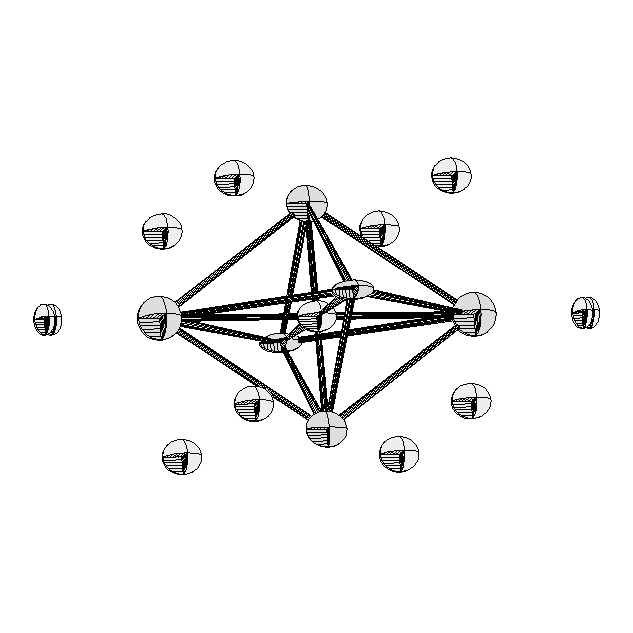
\includegraphics[scale=0.65, angle=0]{fil.1.eps}
   \caption[ATOMS structure plot example]
           {ATOMS structure plot displaying thermal ellipsoids.}
   \label{fil_fig1}
\end{figure}

The structure file saved by {\it DISCUS} contains all atom positions
generated by the space group $Fm\overline{3}m$. The output file
containing the expected eight atoms is listed below:

\begin{MacVerbatim}
    title GaAs
    spcgr F-43m
    cell    5.6537    5.6537    5.6537   90.0   90.0   90.0
    ncell   1,1,1, 8
    atoms
    GA     0.0000    0.0000    0.0000      1.000
    GA     0.0000    0.5000    0.5000      1.000
    GA     0.5000    0.0000    0.5000      1.000
    GA     0.5000    0.5000    0.0000      1.000
    AS     0.2500    0.2500    0.2500      1.000
    AS     0.2500    0.7500    0.7500      1.000
    AS     0.7500    0.2500    0.7500      1.000
    AS     0.7500    0.7500    0.2500      1.000
\end{MacVerbatim}

Note that this version of the file contains the {\tt ncell} keyword.
This example was quite simple since all the atoms are on special
positions and only the F-centering is applied. However, when dealing
with atoms on general positions in a high symmetry space group using
{\it DISCUS} to generate all symmetrically equivalent positions is a
real time saver.

%------------------------------------------------------------------------

\section{Exporting structures \label{file_export}}

{\it PDFFIT} can also export the structure in a format using the
command {\tt save atoms,1,file} (assuming phase number 1 to be
saved). This file can be imported by the structure plotting program
{\it ATOMS} \citep{prog;atoms} using the menu {\it File
$\rightarrow$ Import File $\rightarrow$ Free-Form (.INP)}. An
example displaying thermal ellipsoids can be seen in Figure
\ref{fil_fig1}. The bonds were added in {\it ATOMS}. In order for
{\it ATOMS} to display the complete exported structure, the lattice
parameters and fractional coordinates are adjusted so that the
complete crystal is a single unit cell. Additionally the space group
is set to be $P1$.

%------------------------------------------------------------------------
